\chapter{Magnetism}

Magnets (objects that produce magnetic fields) 

Moving charge (current or moving charges) produce magnetic fields and magnetic fields can only be produced by currents similar to how charges produce electric fields and electric fields can only be produced by charges. It is important to note that even in permanent magnets where there is seemingly not charges moving, the magnetic field is still provided by moving charges (provided by the electron spins of well aligned molecules in this case). Magnetic fields exert forces on currents similar to how electric fields exert forces on charges.

\section{Notation}

Note that $\otimes$ (or $\times$) represents current flowing into the page and $\odot$ represents current flowing out of the page. $\vec{B}$ is used to denote the magnetic field.

\section{Interactions}

\subsection{Laws}

Magnetic fields are similar to other fields where the resultant field at some point in space can be written as the vector sum of all magnetic fields at that point. In other words, magnetic fields follow superposition.

Magnetic fields created by currents/moving charges come in loops perpendicular to the direction of current/moving charge and can be memorized with the right hand rule (shown below).

\hfil 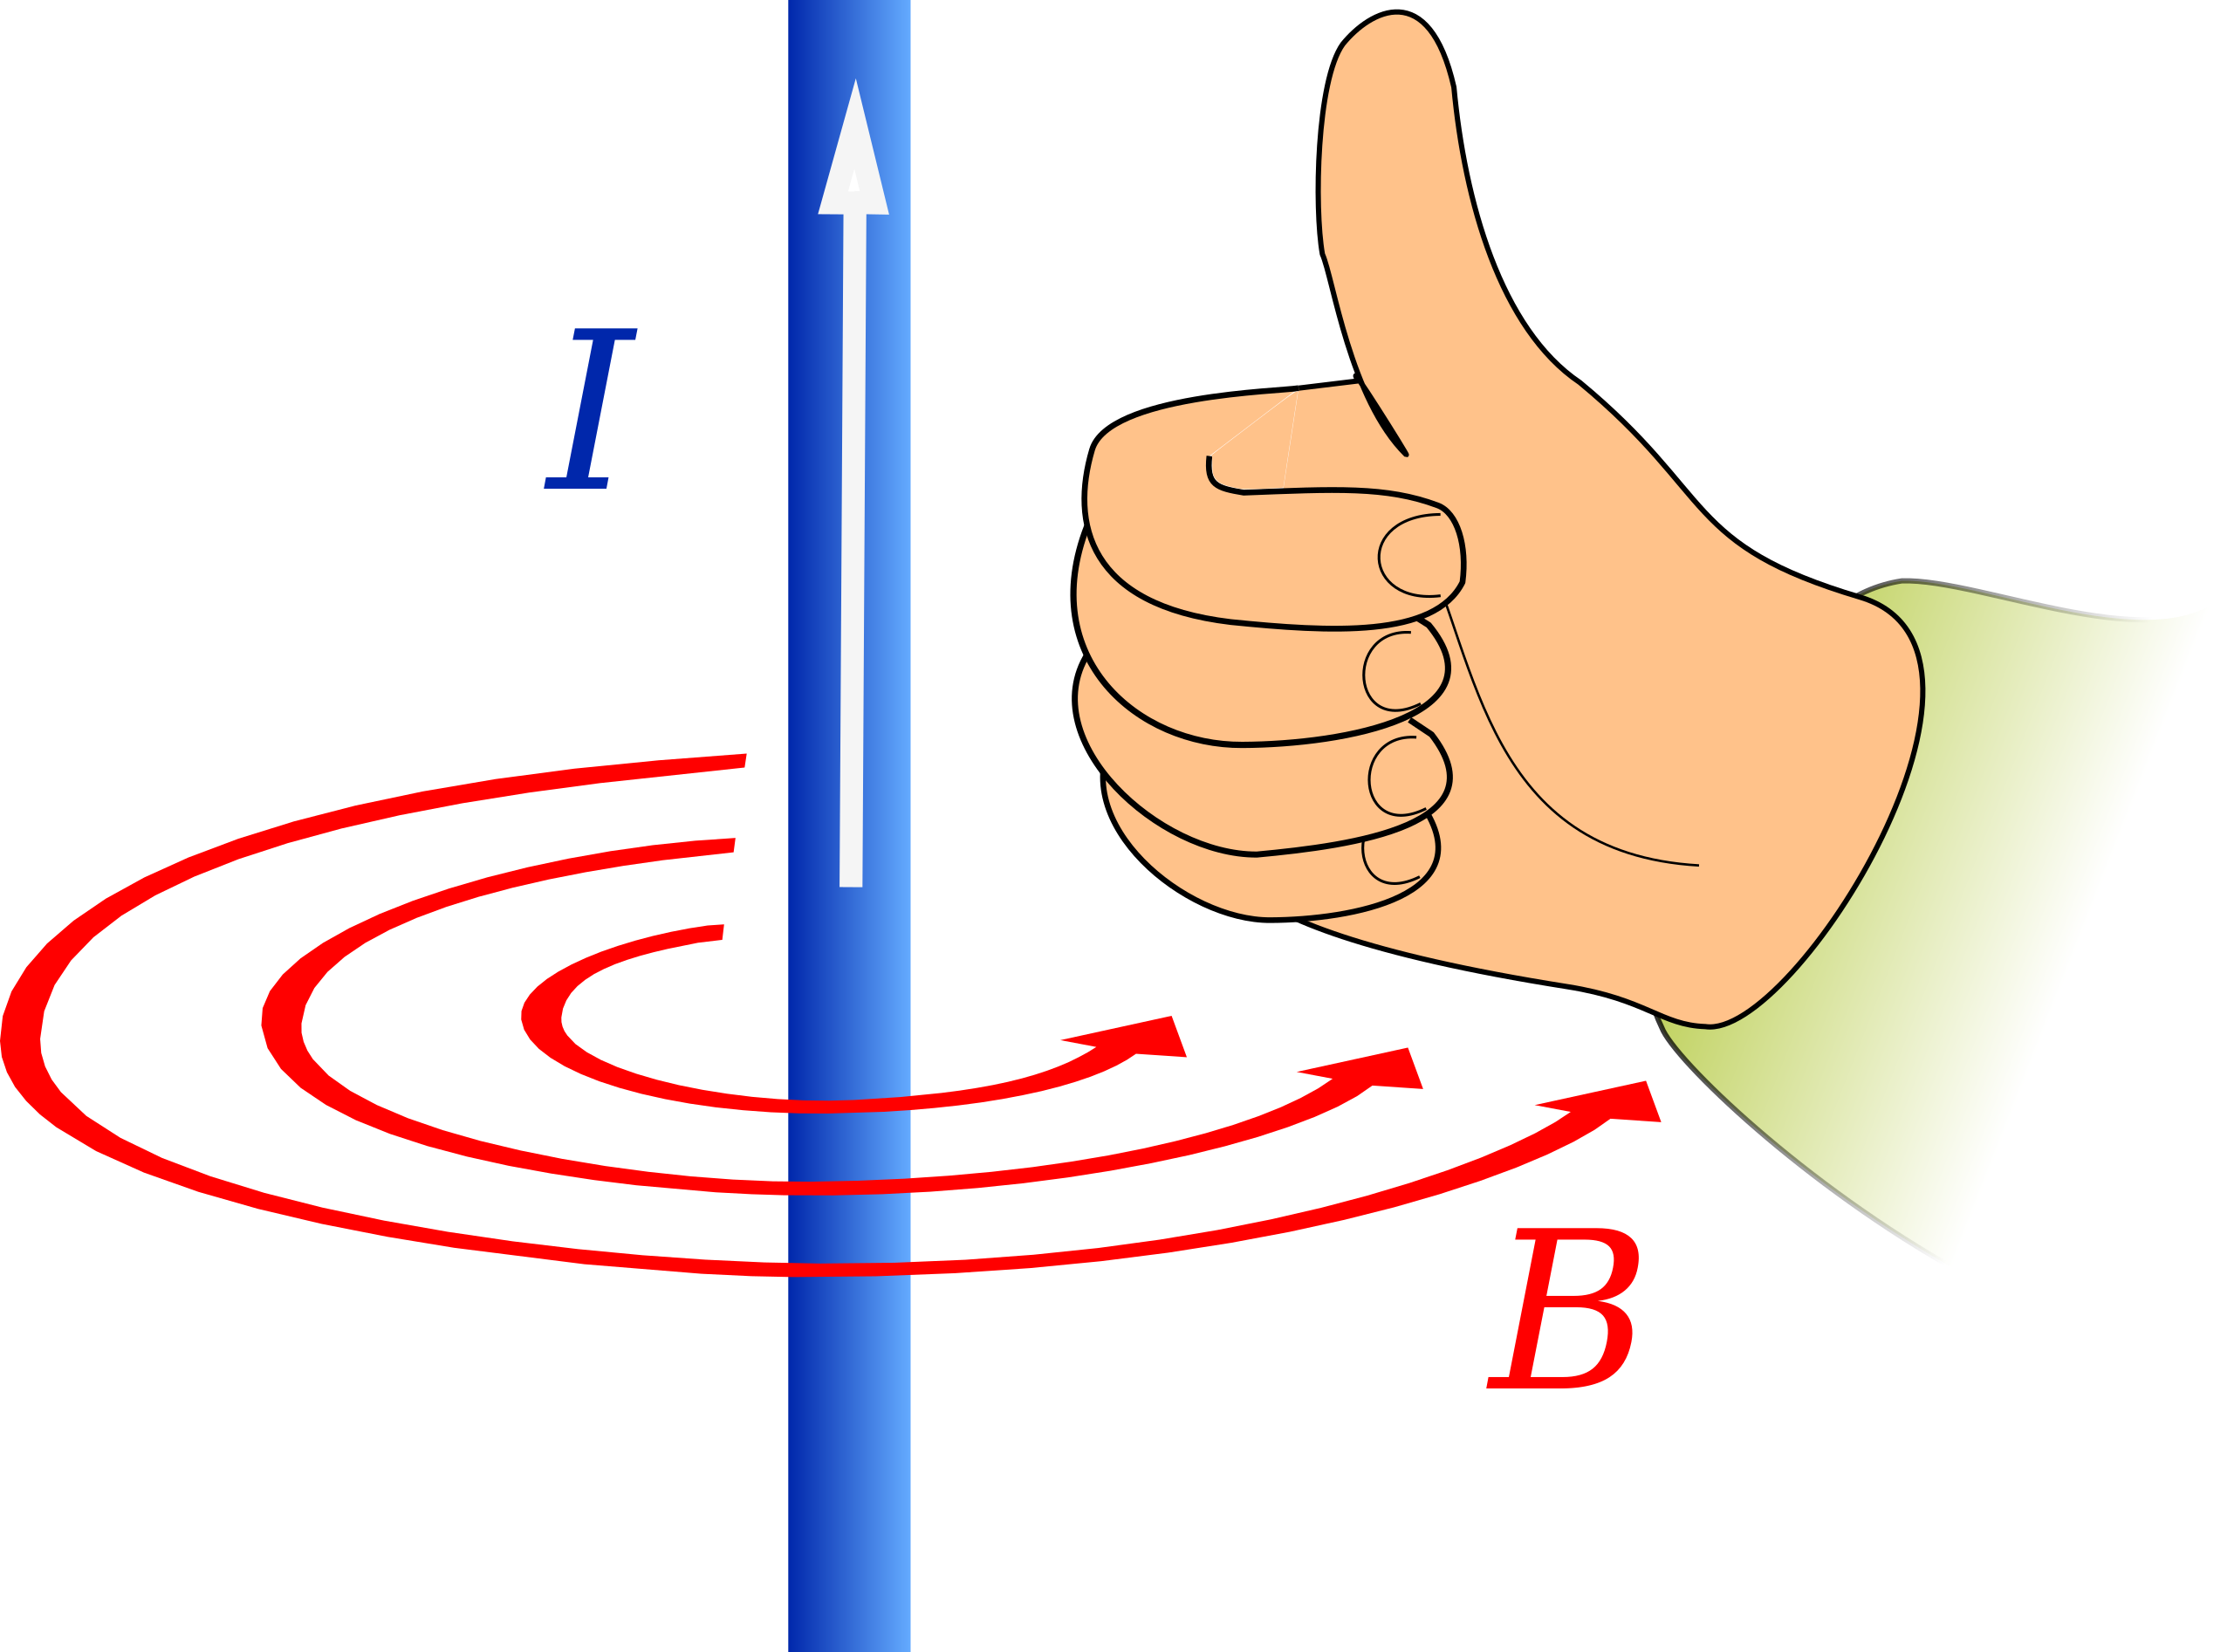
\includegraphics[scale=0.05]{assets/current-rhr.png}

Magnets form magnetic fields with loops coming out of the north pole and going into the south pole.

\hfil 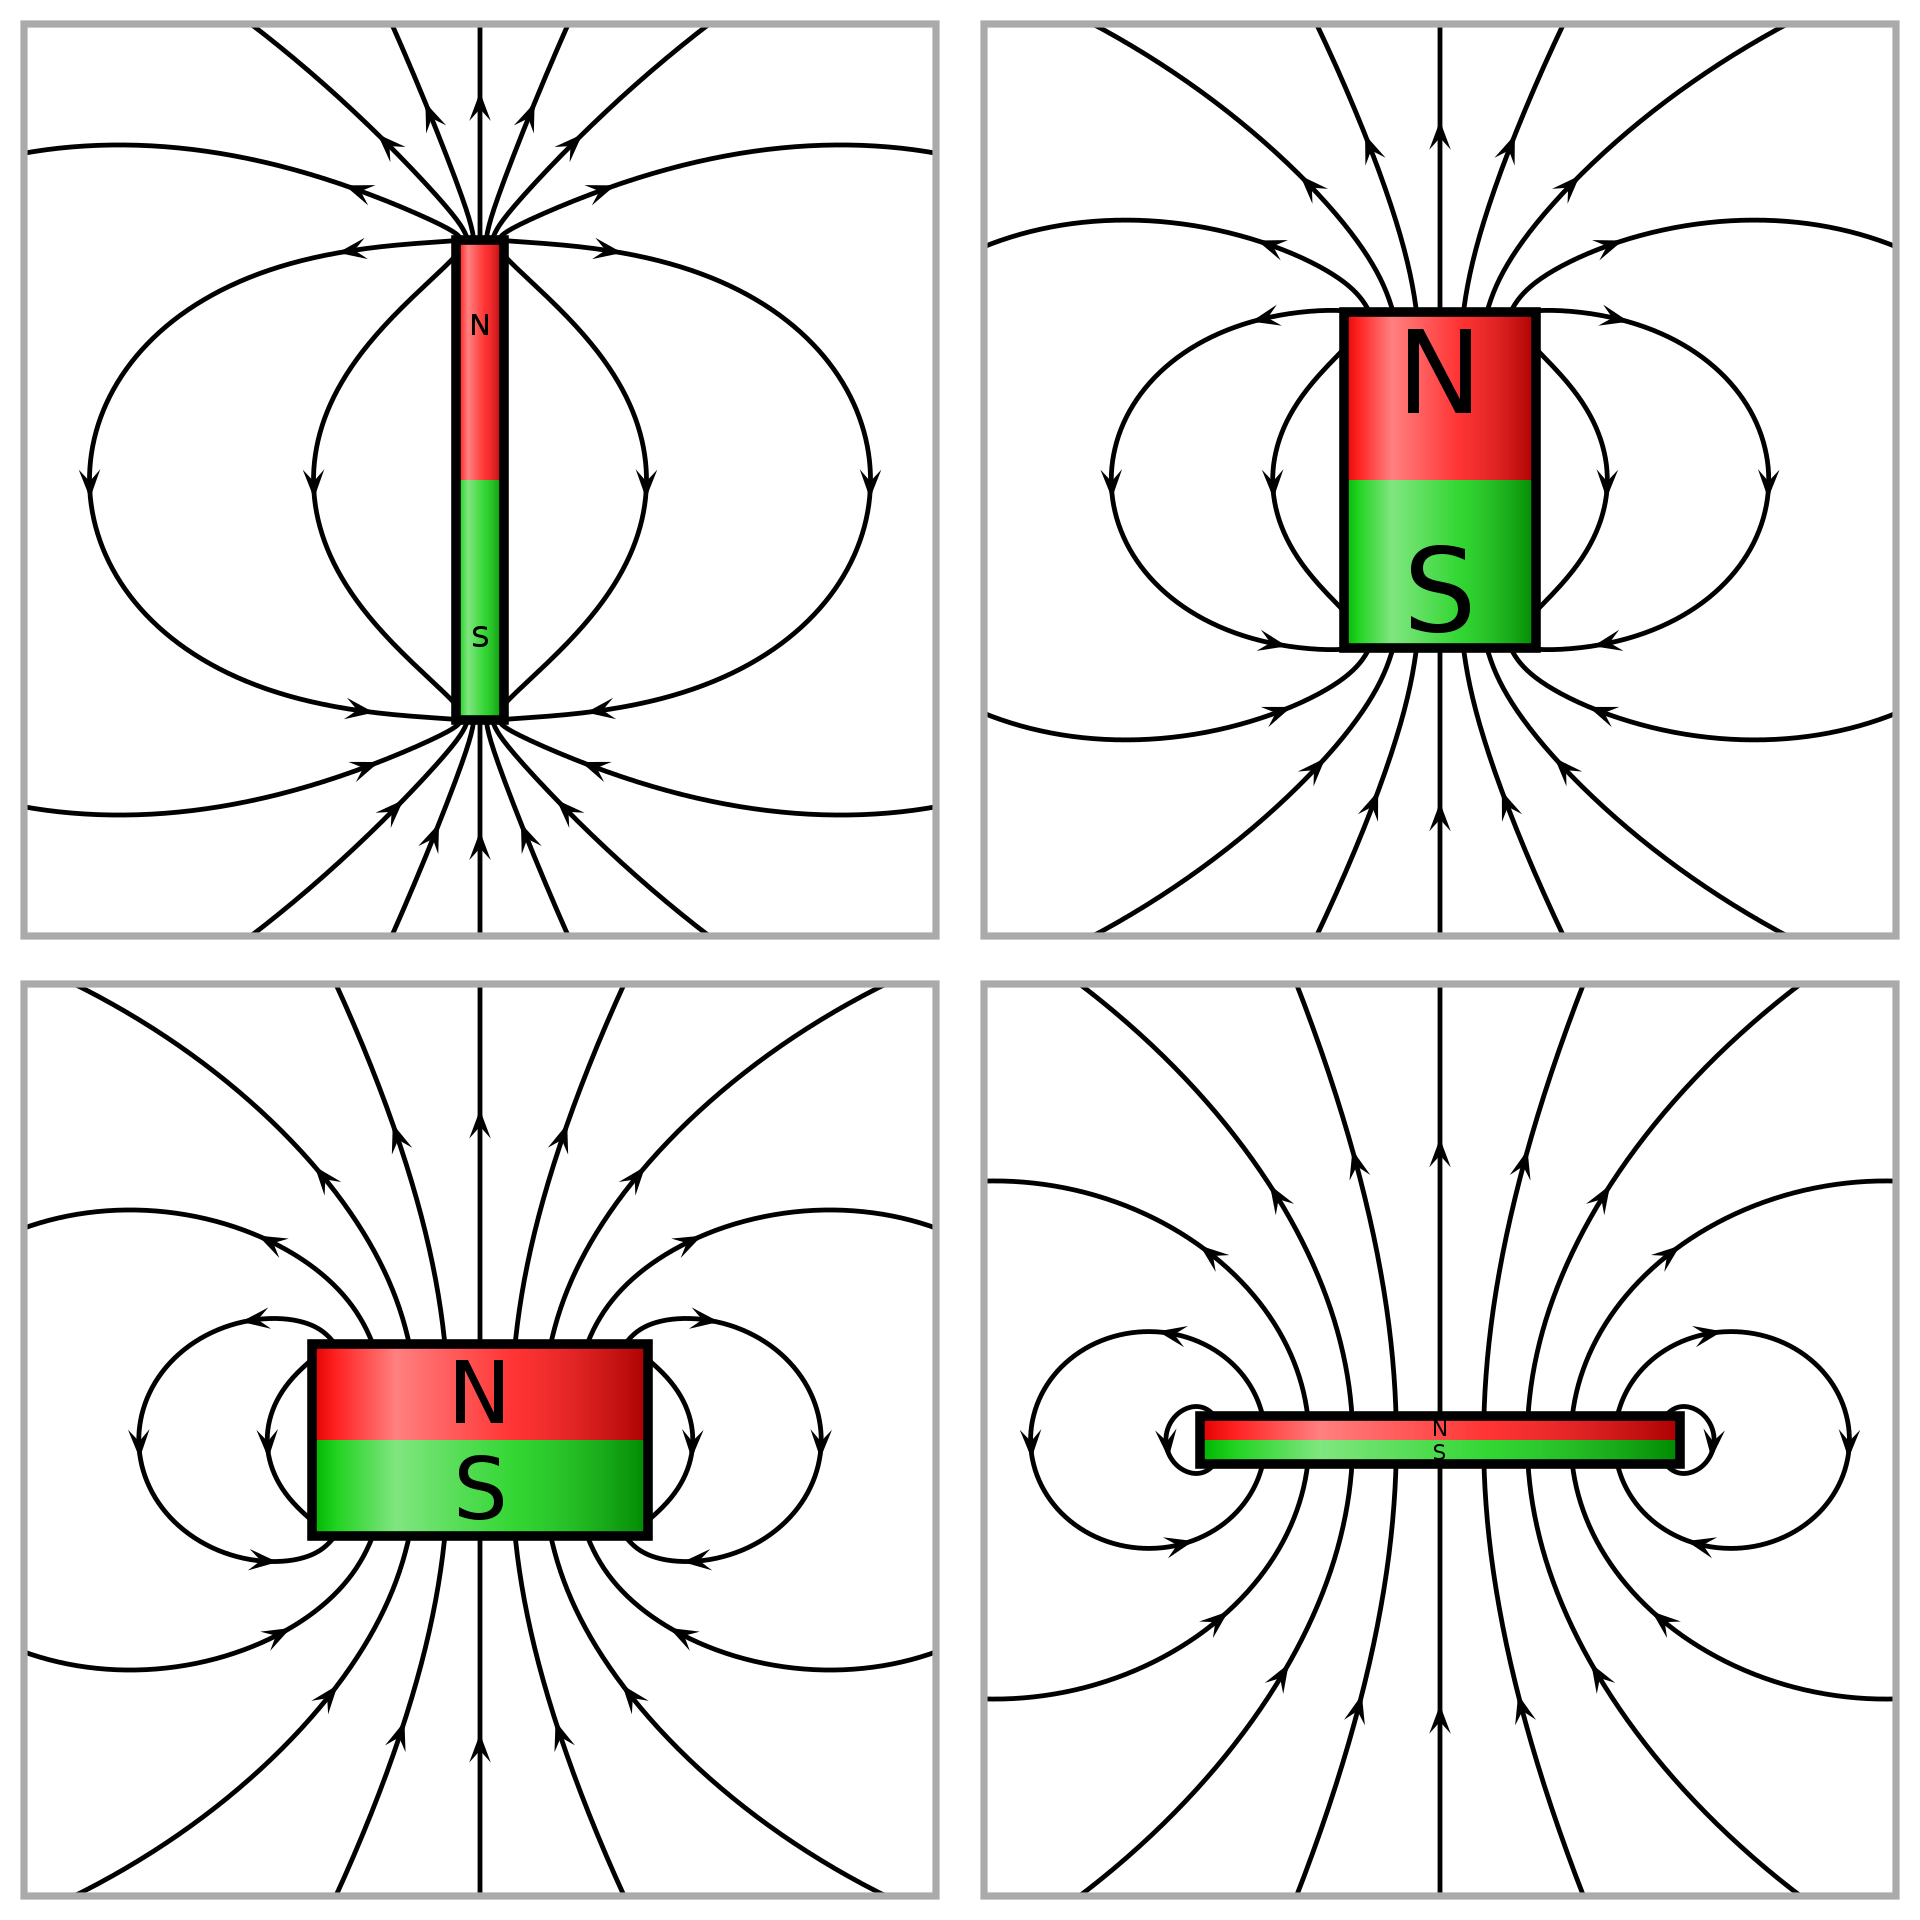
\includegraphics[scale=0.075]{assets/magnets.png}

Since magnetic fields exert force on currents/moving charges, it is necessary to describe the force associated with them: the interaction.

The force experienced by moving charges or currents in magnetic fields are described by the following relations.

\[\vec{F} = q\vec{v}\times\vec{B} \qquad \vec{F} = I\vec{l}\times\vec{B} \qquad \vec{F} = q(\vec{E} + \vec{v}\times\vec{B})\]

On the left is the force exerted on moving charges -- notice how force is only exerted when the charge is moving with non-zero velocity. The middle describes the force exerted on a current. It might be easier to think of the direction of the force with the direction of the current instead of the length of the current. The right presents an equation for the electromagnetic forces exerted on a point charge.

\[\mathbf{F} = q\mathbf{v}\mathbf{B}\sin\theta \qquad \mathbf{F} = I\mathbf{l}\mathbf{B}\sin\theta\]

It is worth noting that the cross product is hard to calculate, and most of times we use the trig equivalent of the expression for calculations, as shown above.

\hfil 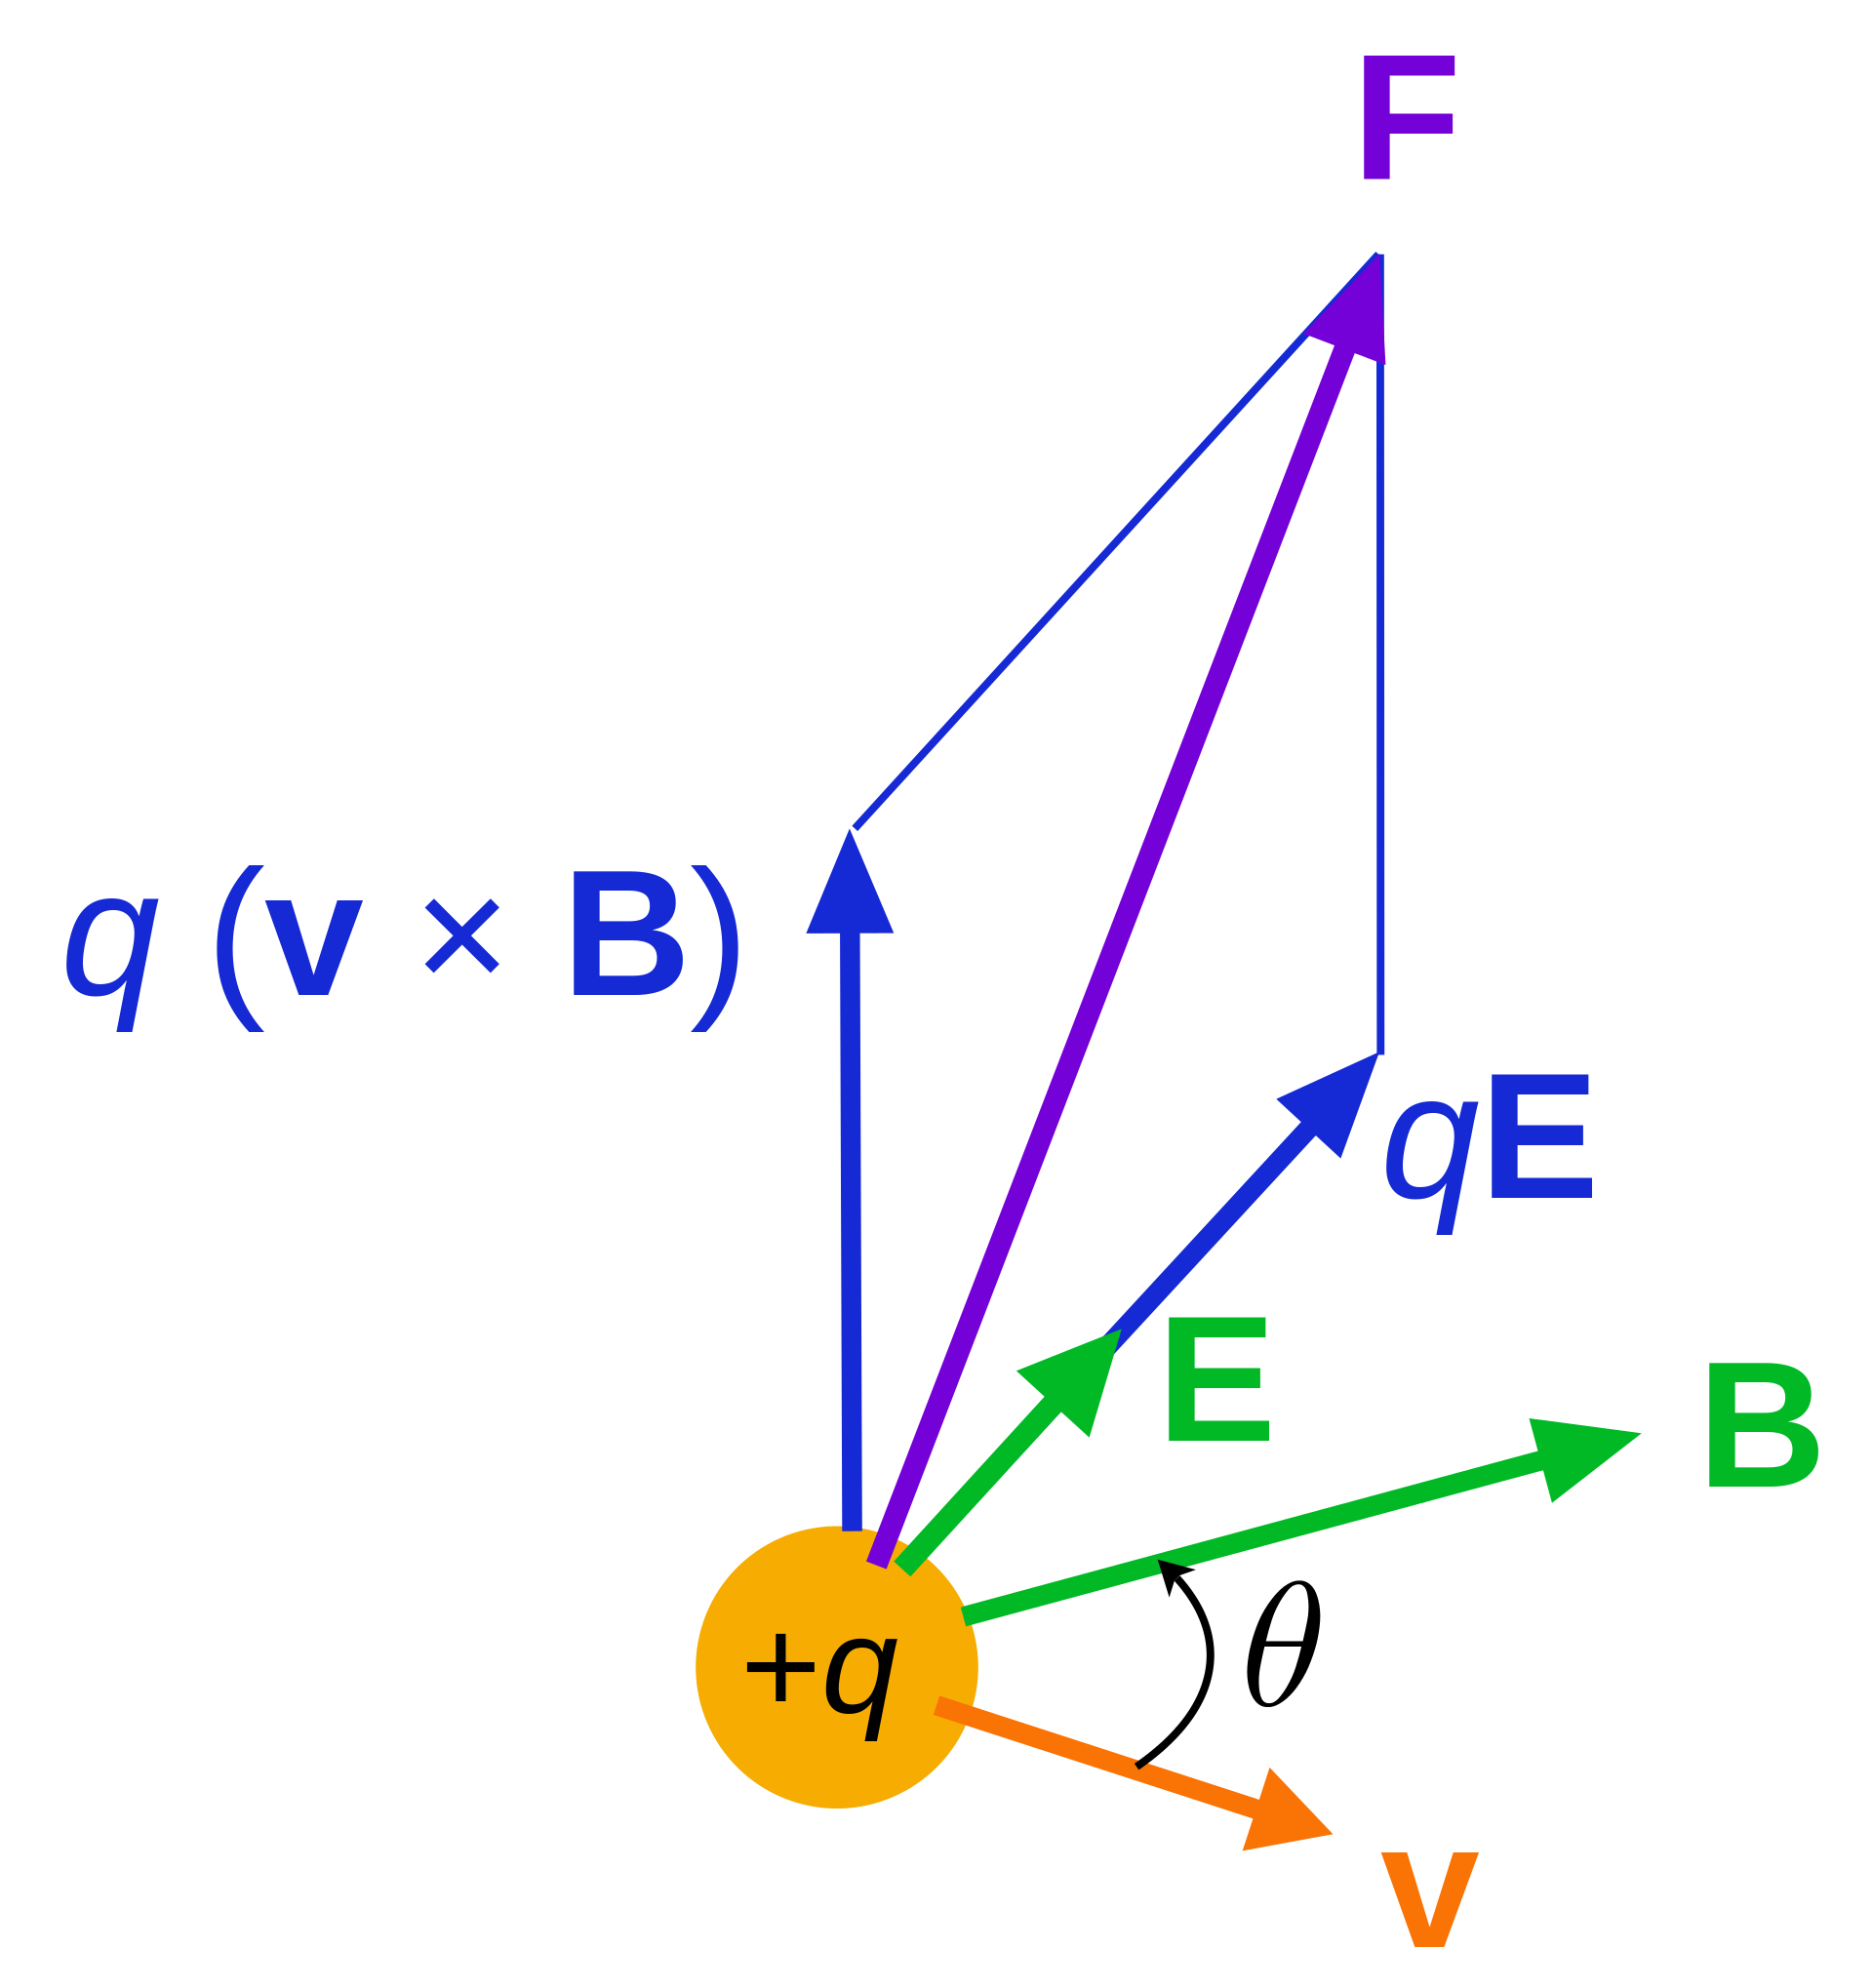
\includegraphics[scale=0.075]{assets/lorentz-force.png}

We can use the right hand rule for thinking about the direction of the cross product. This also implies that the force is always perpendicular to the direction of the magnetic field and the velocity vector. The force is also perpendicular to the magnetic field and the current passthrough. 

\subsection{Applications}



\section{Gauss's Law for Magnetism \& Ampere's Law}

Similar to the electric field, Gauss came up with another law for magnetic fields.

\[\oiint_S B\cdot\mathrm{d}S = 0\]

To understand why this is true, consider the following current loop (or any magnet)

\hfil 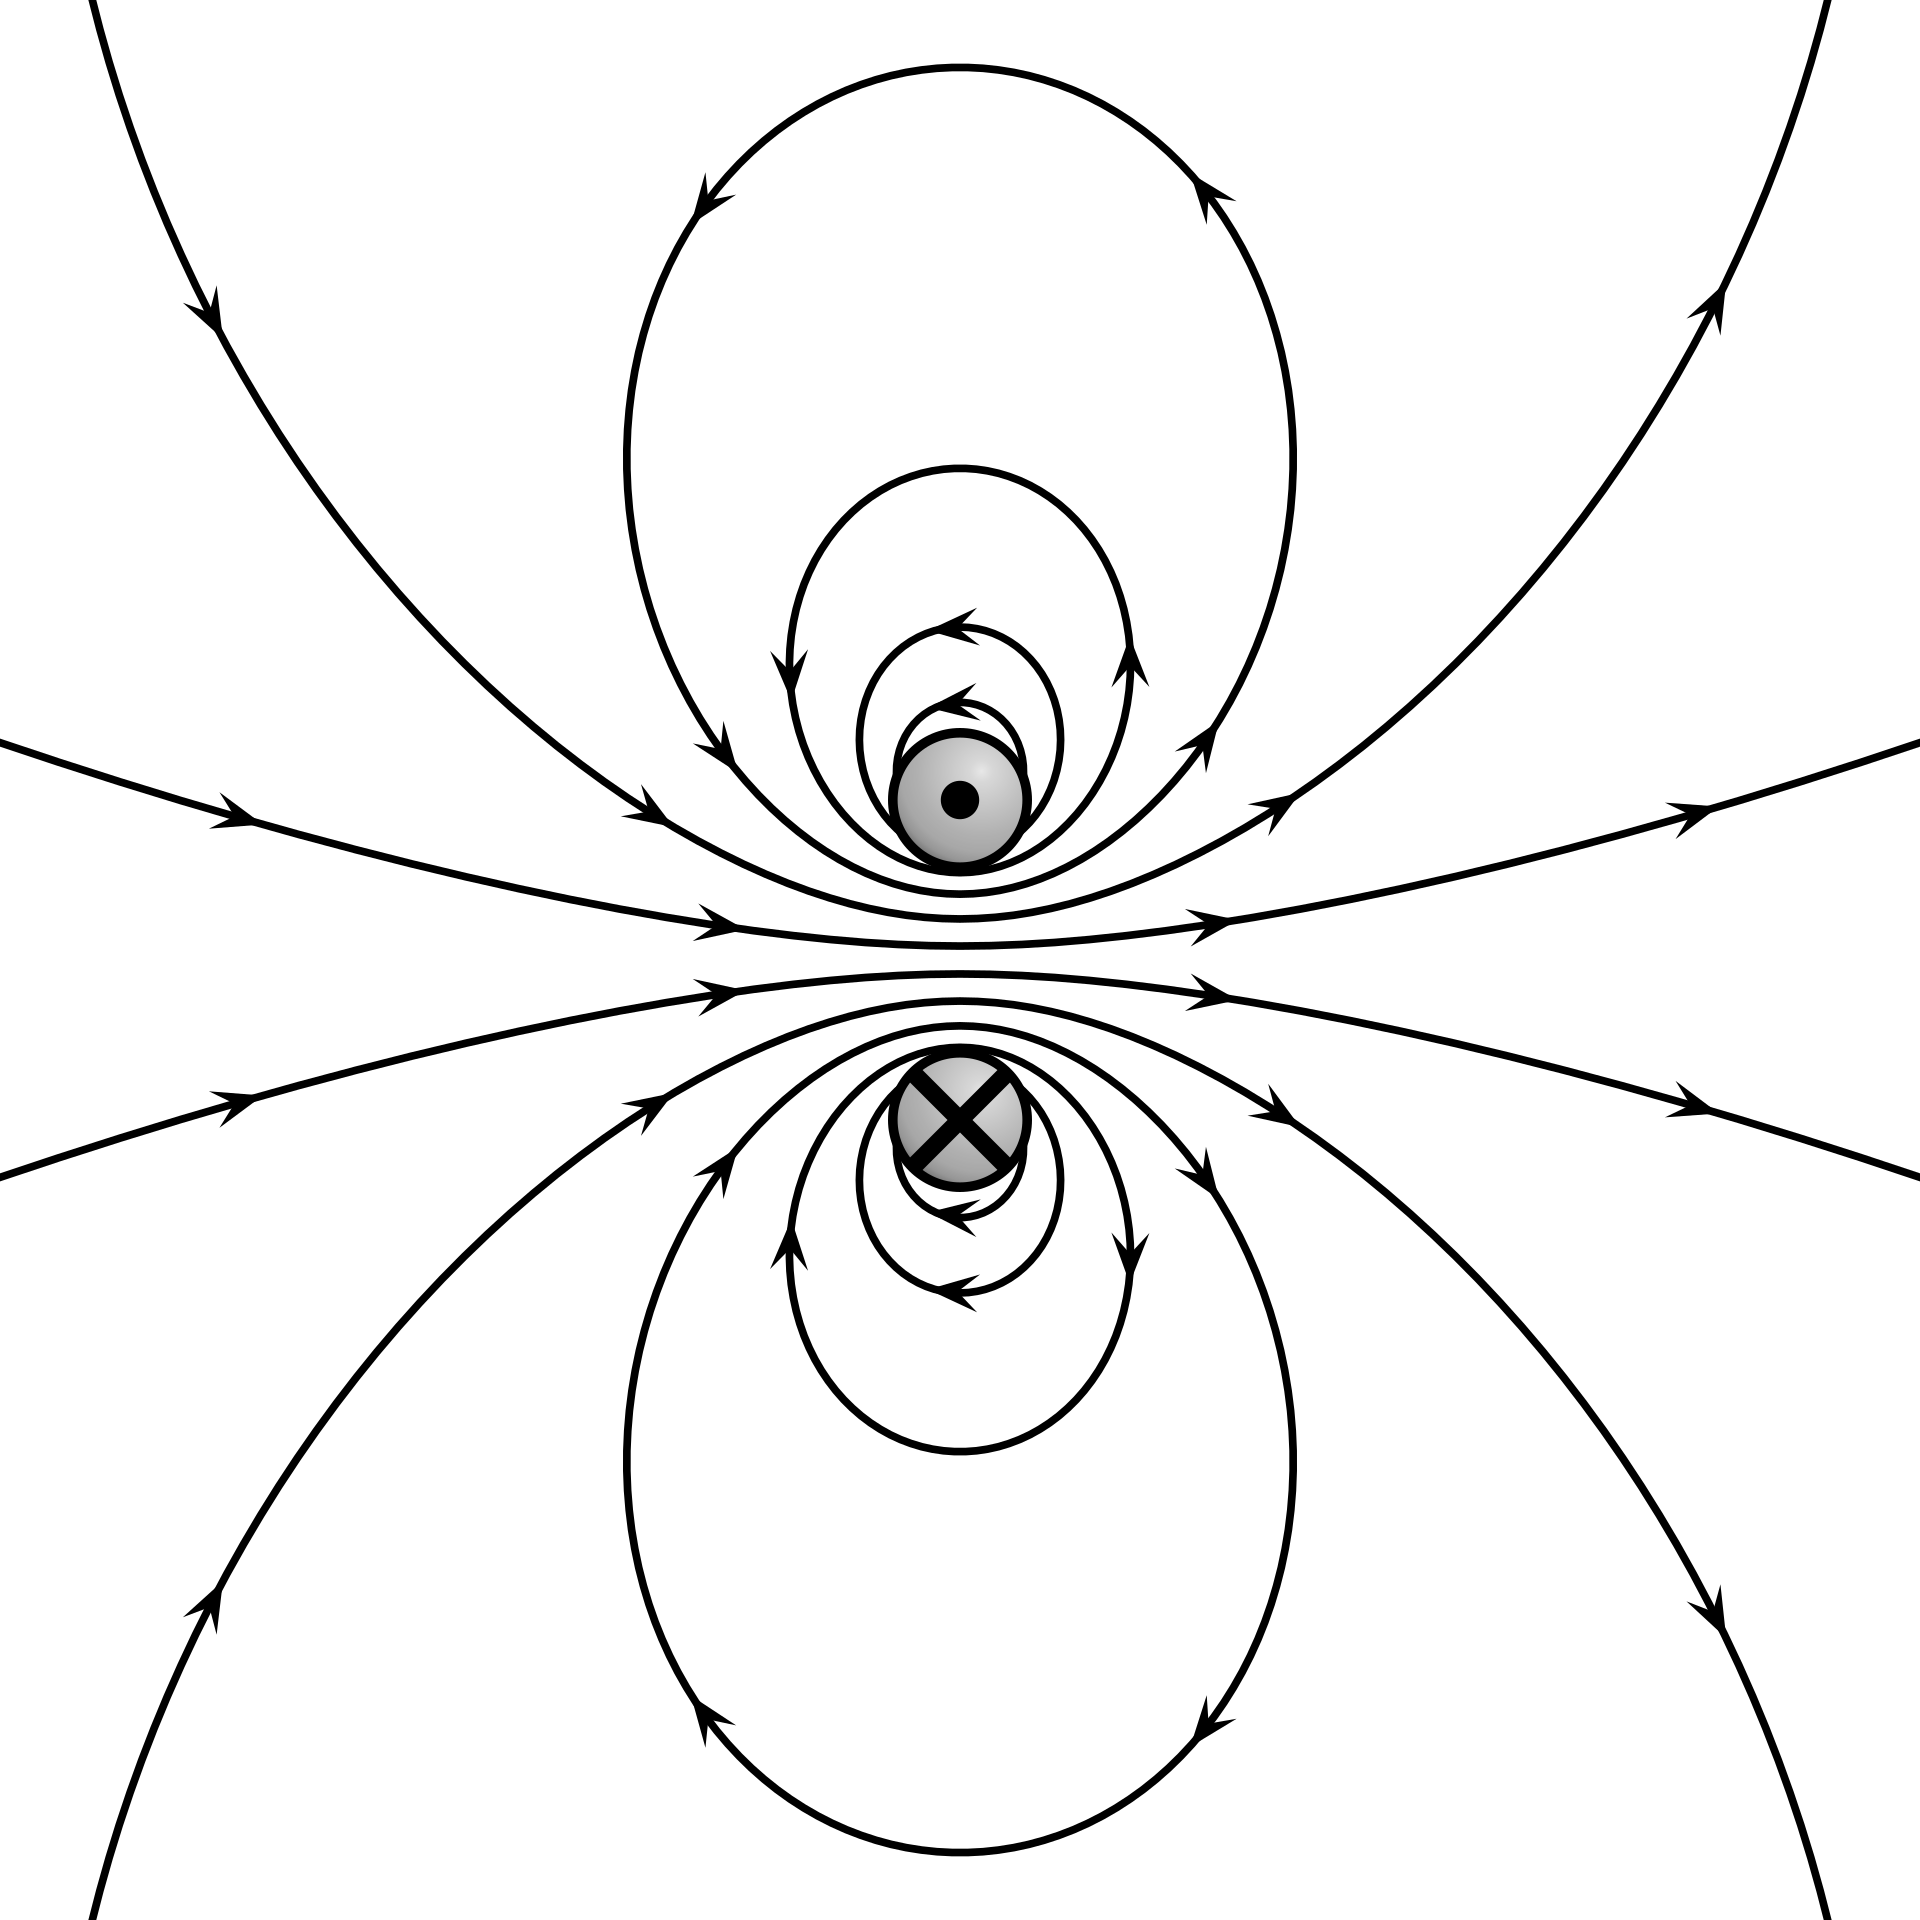
\includegraphics[scale=0.05]{assets/mag-i-loop.png}

When we form a close surface and trace the field lines of the magnetic field at any point, we discover that whatever goes out also comes in (in other words, there are no starts or ends for magnetic field lines, they are in the form of loops), making the net magnetic flux out of any closed surface 0 -- intuitively, for every line out, it has to come back in. This relationship is described by \textbf{Gauss's Law for Magnetism}, shown above.

Then there is \textbf{Ampere's Law}:

\[\oint_C B \cdot \,\mathrm{d}l = \mu_0 I_{\mathrm{enc}}\]

\hfil in the form that we are concerned with,

where $B$ is the magnetic field, $C$ is the closed path for which we are integrating along, $\mu_0$ is the \textbf{Vacuum Permeability} (value shown below), and $I_{\mathrm{enc}}$ is the amount of current passing through the surface enclosed by path $C$.

\[\mu_0 = \SI{1.25663706212(19)e-6}{\henry\per\meter}\]

This is similar to Gauss's Law for measuring electric flux out of some gaussian surface. Ampere's Law, combined with Gauss's Law for Magnetism will be helpful in finding the magnetic field of different currents.

\section{Applications of Ampere's Law}

We list a few different scenarios where we can derive the expression for magnetic field utilizing the two rules are described above.

\subsection{Single Long Straight Wire/Current}

\hfil 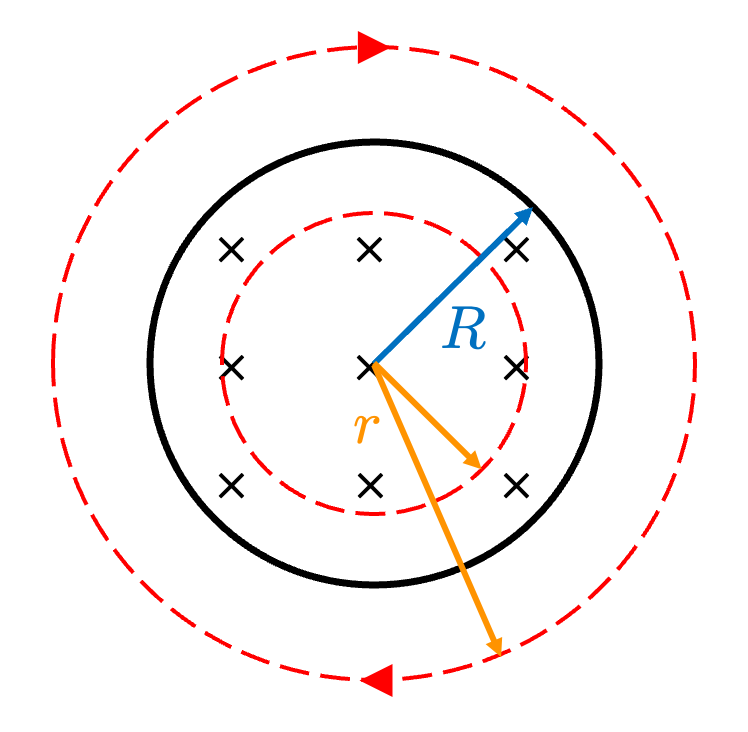
\includegraphics[scale=0.4]{assets/amp-law-single-wire.png}

There are actually two regions that we can consider for a long straight wire: regions inside the wire and regions outside the wire. Let us assume that the wire has a radiums of $R$ and represent our magnetic field at some radius $r$ as $B$.

First for $r > R$:

\dots

Now, $r < R$:

\dots


\subsection{Sheet of Wires/Currents}

\hfil 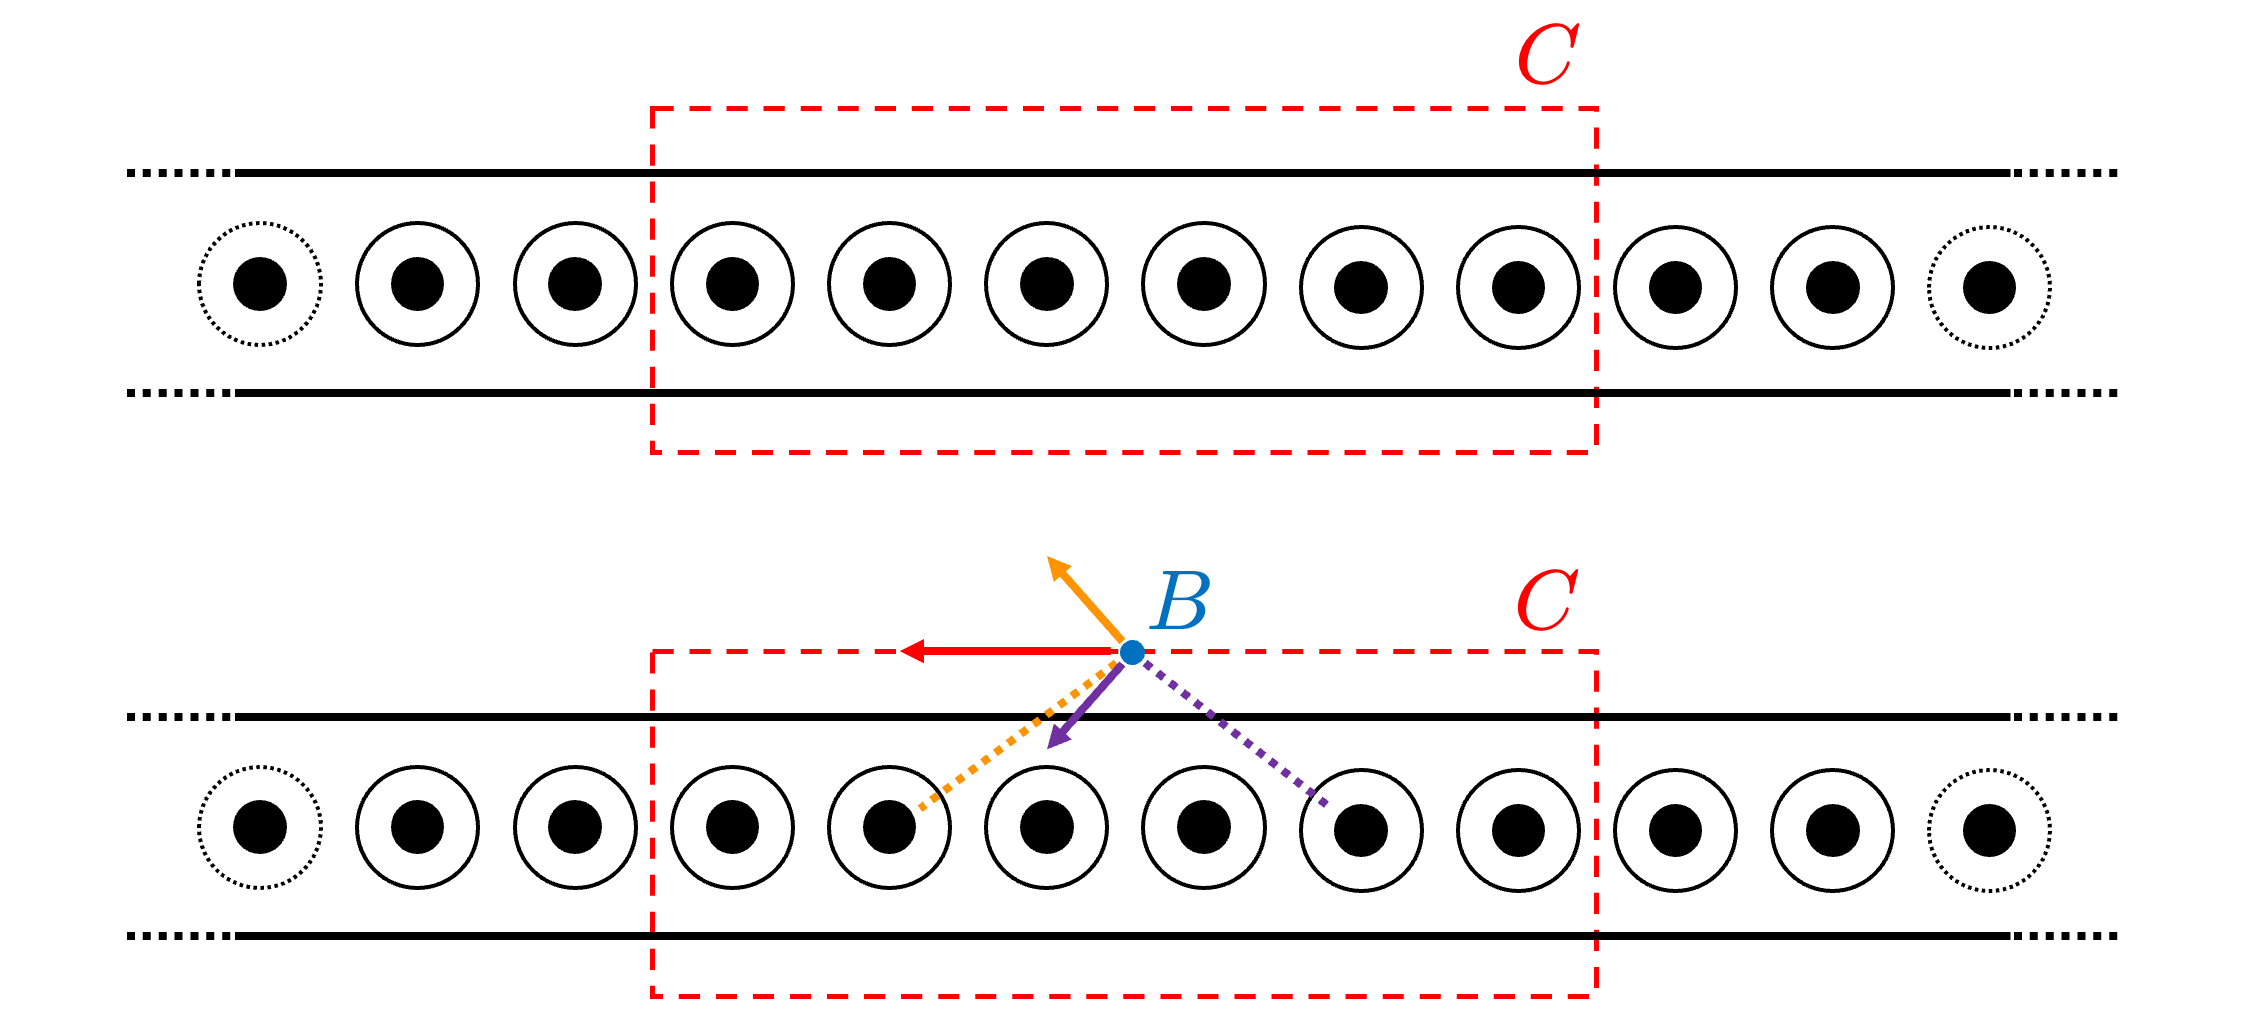
\includegraphics[scale=0.15]{assets/amp-law-current-sheet.png}

Now that we have considered a single straight wire, we can also consider a sheet of current/wires and the magnetic field that this creates.

\subsection{Solenoids}

\hfil 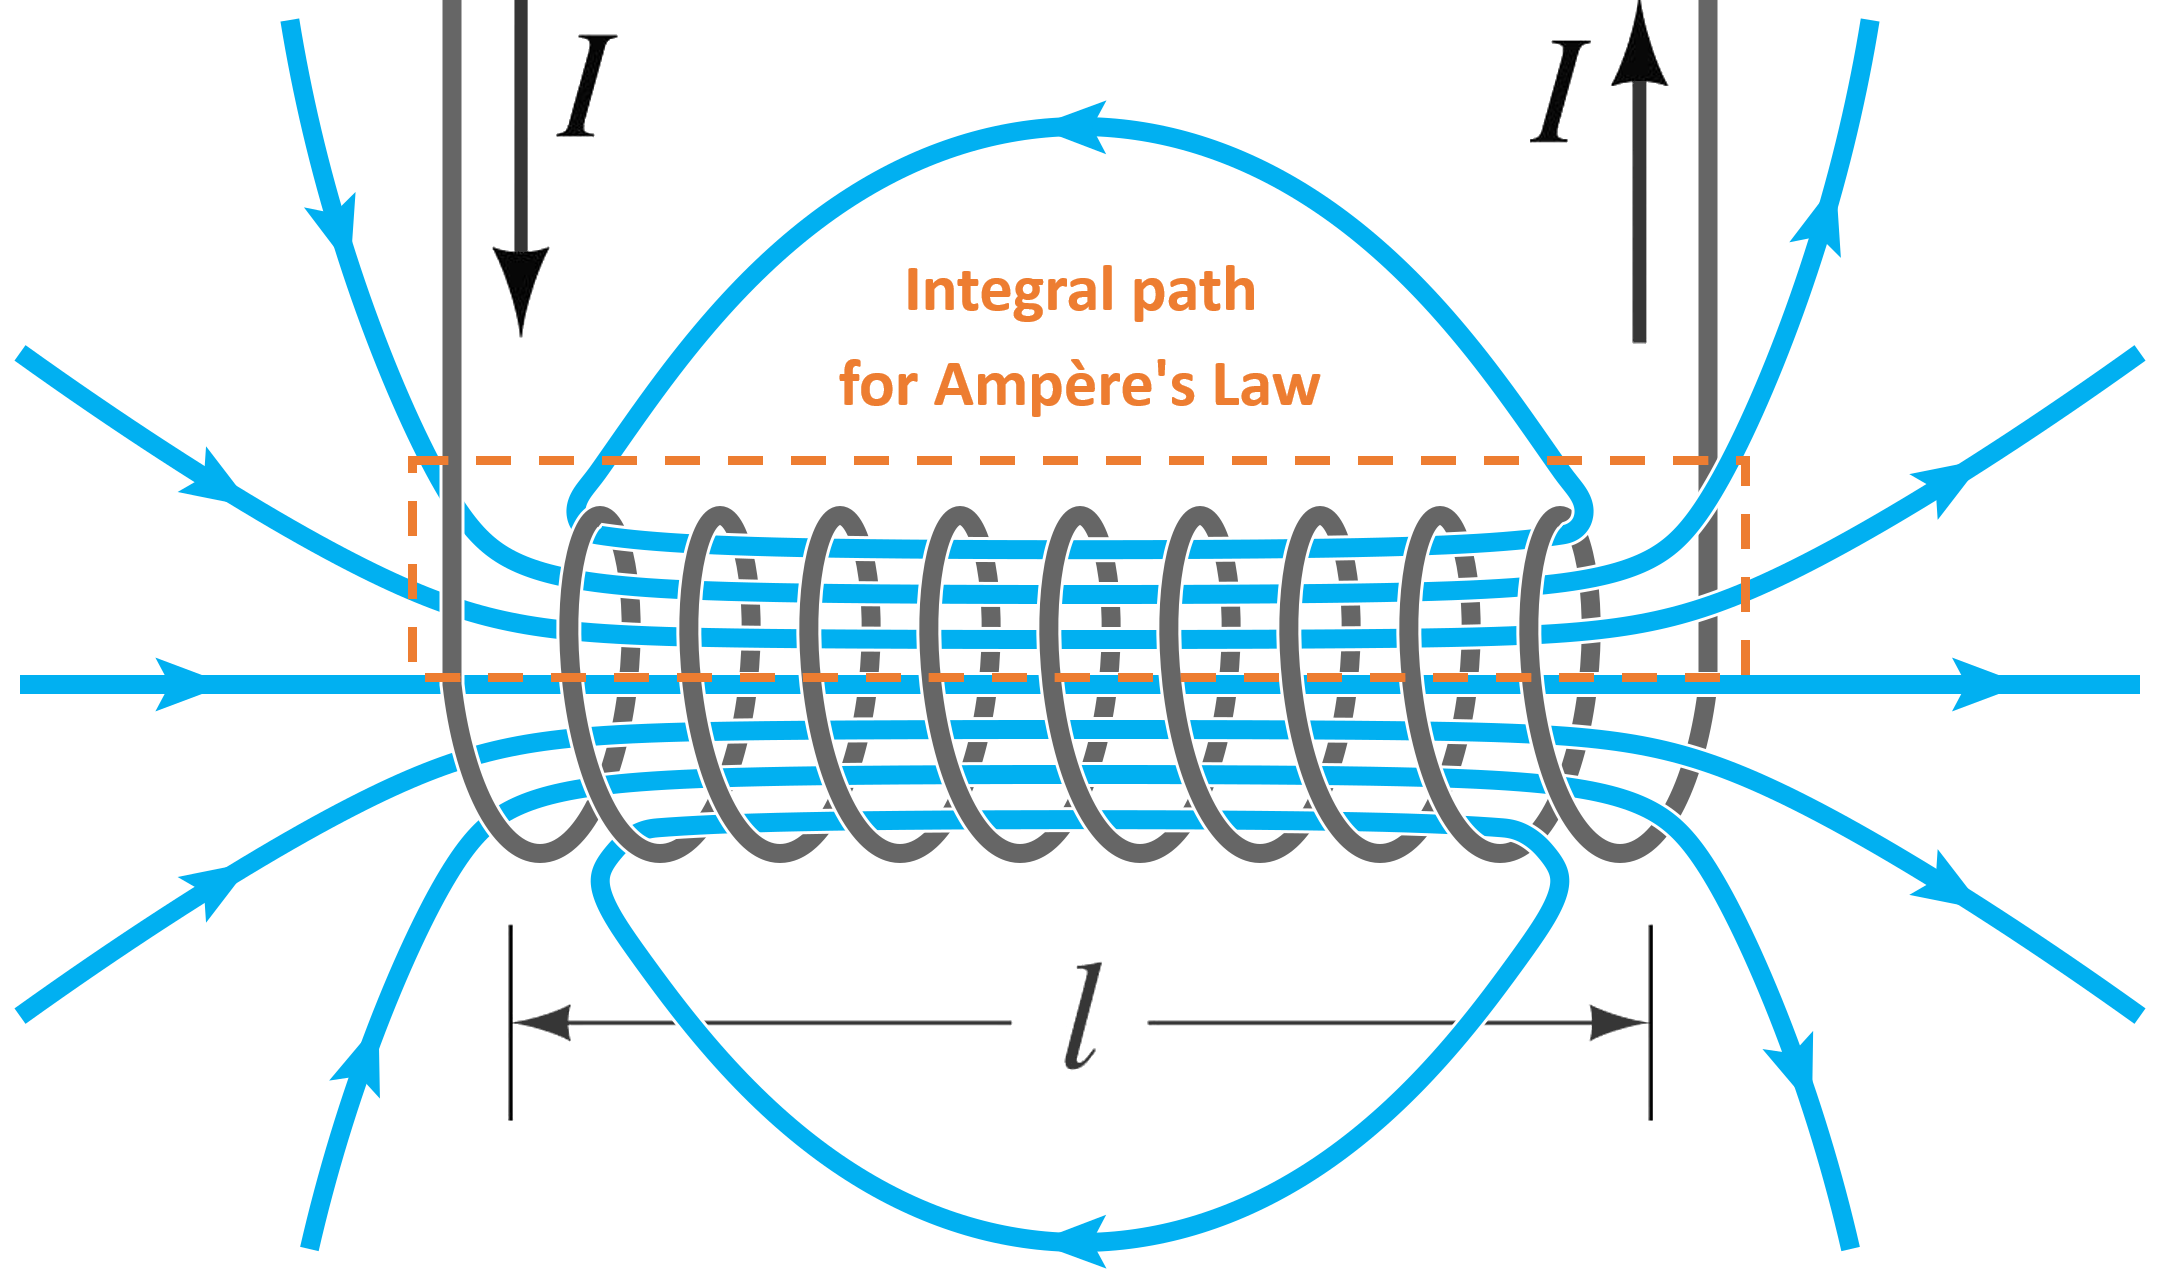
\includegraphics[scale=0.1]{assets/amp-law-solenoid.png}

For this case we will consider idealized solenoids where we consider the magnetic field outside the solenoid to be 0.

\section{Biot-Savart Law}

\subsection{Law}


\subsection{Moving Charges}


\section{Derivation for Field of Currents}